\documentclass{article}[11pt]
\usepackage[left=1.0in, right=1.0in, top=1.0in, bottom=1.0in,nohead]{geometry}              		
\geometry{letterpaper}

\usepackage{graphicx, grffile}														
\usepackage{amssymb, amsmath, amsfonts}
\usepackage{setspace}
\usepackage{titlesec}
\usepackage[usenames, dvipsnames]{color}
\usepackage{soul}
\usepackage{float, multirow, tabulary}
\usepackage{subcaption}

\newcommand{\bp}[1] {\left( #1 \right)}
\newcommand{\bb}[1] {\left[ #1 \right]}
\newcommand{\ba}[1]{\left| #1 \right|}
\newcommand{\infint}{\int_{-\infty}^\infty}

\titleformat{\section}{\Large\bfseries}{\thesection}{0.5em}{}
  
\titleformat{\subsection}{\normalfont\normalsize\bfseries}{\thesubsection}{0.5em}{}

\titleformat{\subsubsection}{\normalfont\normalsize\bfseries\itshape}{\thesubsubsection}{0.5em}{}  
  
\titlespacing{\section}{0pt}{0pt}{2pt}

%\newcommand{\kbcom}[1]{
%\textcolor{blue}{\textbf{\textit{\ul{#1}}}}}
%
%\newcommand{\blcom}[1]{
%\textcolor{red}{\textbf{\textit{\ul{#1}}}}}         
%
%\newcommand{\llcom}[1]{
%\textcolor{Orange}{\textbf{\textit{\ul{#1}}}}}
%
%\newcommand{\tlcom}[1]{
%\textcolor{LimeGreen}{\textbf{\textit{\ul{#1}}}}} 

\newcommand{\Matlab}{\textsc{Matlab}}

\title{Final Report on Parameter Estimation for Nonlinear Dynamical Systems}
\author{Brett Larsen and Ajay Karpur}
\date{}


%%%

\begin{document}
\maketitle
\doublespace

%\vspace{-30pt}

\begin{abstract}
The purpose of this project was to explore the methods by which one could estimate the values of parameters underlying a nonlinear dynamical system. To accomplish this, we examined the parameter $\beta$ underlying a simulation of the Lorenz system in \Matlab.
\end{abstract}

\section{Introduction}
\label{sec:intro}
In estimation theory, parameter estimation is used to determine approximate values of parameters from a set of measured data that have some degree of randomness. By estimating the value of these parameters, one can approximate the conditions underlying some system. Parameter estimation has applications in a variety of engineering problems. When mathematical models are used to describe biological or other nonlinear dynamical phenomena, these models often contain some parameters that cannot be directly quantified or calculated. In these cases, the parameters can be estimated using the available data.


%%%%%%%%%%%%%%%%%%%%%%%%%%%%%%%%%%%%%%%%%%%%%%%%%%%%%%
%\vspace{-10pt}
%\section{Background}
%\label{sec:background}

\section{Background}
\label{sec:intro}
The Lorenz system is a set of three ordinary differential equations used originally by Edward Lorenz as a model of convection in the atmosphere.  The three equations are as follows:

\begin{equation}
	\frac{dx}{dt} = \sigma (x - y)
\end{equation}
\begin{equation}
	\frac{dy}{dt} = x (\rho - z) - y
\end{equation}
\begin{equation}
	\frac{dz}{dt} = xy - \beta z
\end{equation}

Thus, the Lorenz system has three parameters, $\sigma$, $\rho$, and $\beta$.  The Lorenz system is particularly intriguing because of its chaotic behavior.  Although the system in deterministic, small changes in the initial condition, can cause large changes in the eventual evolution of the system.  Beyond Lorenz's original work, the Lorenz system has found to be effective in modeling a number of other physical systems, including electrical circuits and lasers.

Another interesting aspect of the Lorenz system is its strange attractor.  An attractor is a mathematical structure to which a dynamical system tends to evolve no matter how the system is started.  In the case of a 3-dimensional system like the Lorenz system, the attractor can be plotted.  What makes the Lorenz system attractor unique is that it has a fractal structure and is thus designated a strange attractor.  A particularly famous case is the one that results from the initial conditions $\sigma$ = 10, $\rho$ = 28, and $\beta$ = 8/3.  The plotted attractor is shown in .  Strange attractors often occur in chaotic systems.

The purpose of this project is to examine the sensitivity of the Lorenz system and functions of the data points generated by the Lorenz system to certain parameters, in this case $\beta$.
%%%%%%%%%%%%%%%%%%%%%%%%%%%%%%%%%%%%%%%%%%%%%%%%%%%%%%
%\vspace{-10pt}
\section{Methods}
\label{sec:methods}

To acquire random data, we used a \Matlab \ simulation of the Lorenz system.


%%%%%%%%%%%%%%%%%%%%%%%%%%%%%%%%%%%%%%%%%%%%%%%%%%%%%%
%\vspace{-10pt}
\section{Results}
\label{sec:results}

\begin{figure}[H]
\centering
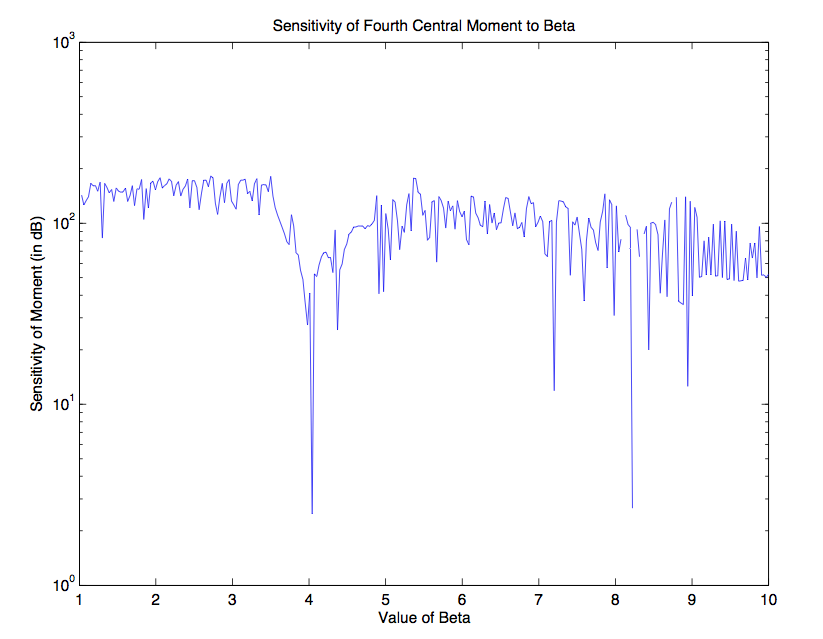
\includegraphics[scale = 0.6]{SensitivityFourth.png}
\caption{Example of an WD TFR}
\label{fig:WDTFR}
\end{figure}
\begin{figure}[H]
\centering
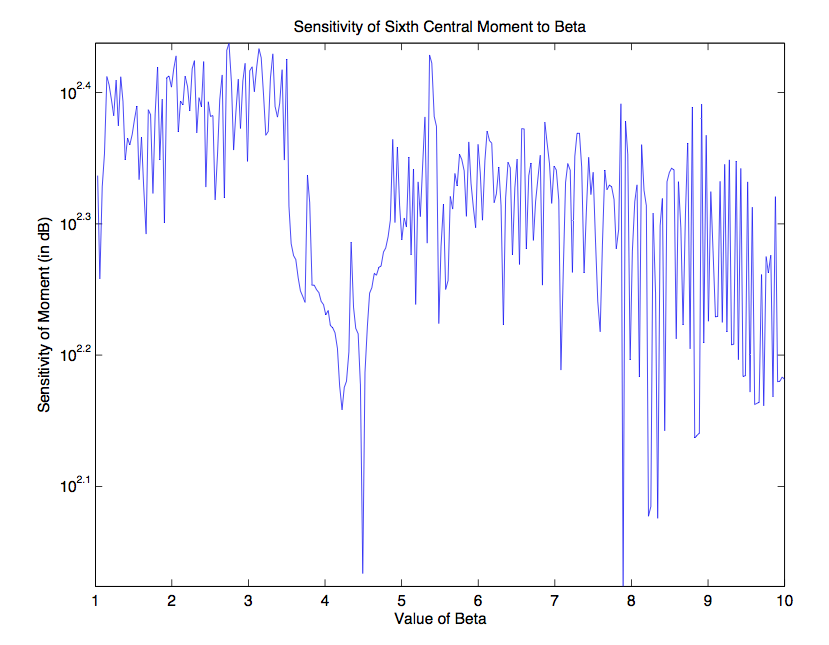
\includegraphics[scale = 0.6]{SensitivitySixth.png}
\caption{Example of an WD TFR}
\label{fig:WDTFR2}
\end{figure}

%\vspace{-10pt}
\section{Conclusions}
\label{sec:conclusion}


\section{Acknowledgements}
\label{sec:Ack}
We would like to acknowledge Moiseev Igor for the open source \Matlab \ Lorenz system generator.


%Bibliography
\bibliographystyle{IEEEtran}
\bibliography{proposal_refs.bib}

\end{document}